\documentclass[a4paper]{article}

%% Language and font encodings
\usepackage[english]{babel}
\usepackage[utf8x]{inputenc}
\usepackage[T1]{fontenc}

%% Sets page size and margins
\usepackage[a4paper,top=3cm,bottom=2cm,left=3cm,right=3cm,marginparwidth=1.75cm]{geometry}

%% Useful packages
\usepackage{amsmath}
\usepackage{graphicx}
\usepackage[colorinlistoftodos]{todonotes}
\usepackage[colorlinks=true, allcolors=blue]{hyperref}

%% Ammar Packages
\usepackage{float}
\usepackage{algpseudocode}


\title{ROB537: HW2}
\author{Ammar Kothari}

\begin{document}
\maketitle

\section{Introduction}
Optimization through search is an important part of modern engineering.  With the advent of modern computers, people are able to generate and evaluate many solutions.  Search has been used widely in fields like engineering and finance, but has also found uses in politics \cite{totenberg_2017}.  Search is an integral part of finding solutions to challenging problems today.

In this assignment, I apply three search algorithms to solve a Travelling Salesman Problem (TSP) with 15, 25, or 100 cities that are dispersed somewhat evenly through the map.  A fourth scenario with 25 cities is structured in a way to make the solution easily identifiable.  The three algorithms investigated are Simulated Annealing, Genetic Algorithms, and Monte Carlo Tree Search.

\section{Problem Description}
TSP is meant to replicate the challenge of a traveller trying to visit many places without revisiting any locations.  Accordingly, the solution must contain every city only once, except for the start location.  The path must start and end at the same location.  The goal is to minimize the total cost of the path.  In this case, the cost is the distance travelled.

%!TEX root = HW2.tex
\begin{figure}[h]
	\centering
	\begin{minipage}{0.5\textwidth}
	    \centering
	    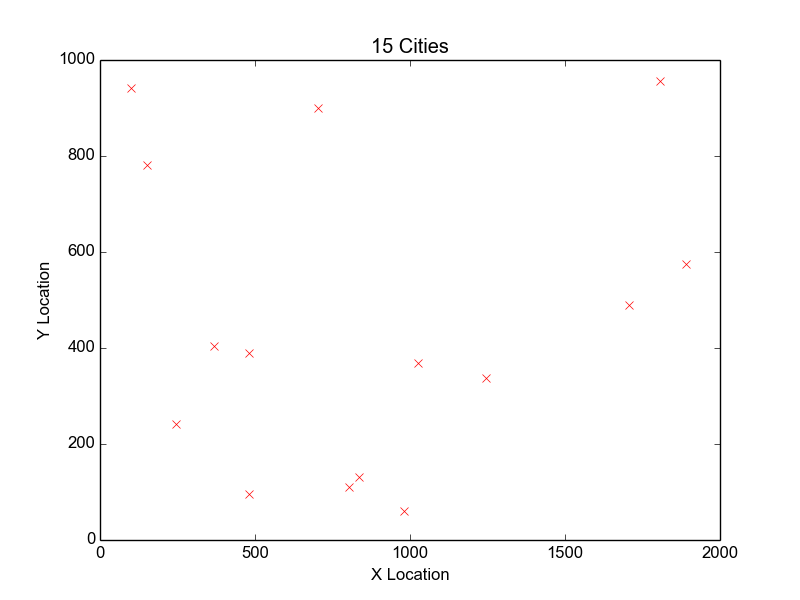
\includegraphics[width=0.9\textwidth]{15cities.png}
	    \caption{15 cities plot}
	    \label{fig:15cities}
    \end{minipage}\hfill
	\begin{minipage}{0.5\textwidth}
	    \centering
	    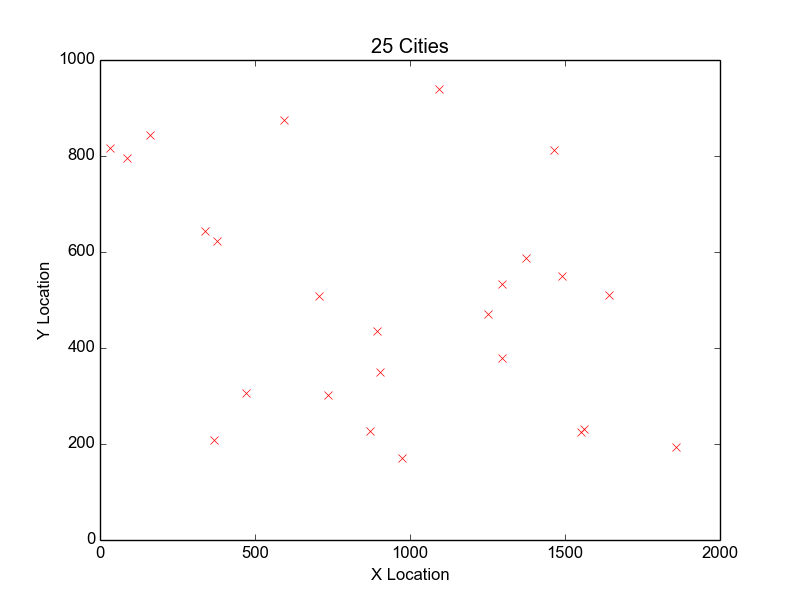
\includegraphics[width=0.9\textwidth]{25cities.png}
	    \caption{25 cities plot}
	    \label{fig:25cities}
    \end{minipage}\hfill
	\begin{minipage}{0.5\textwidth}
	    \centering
	    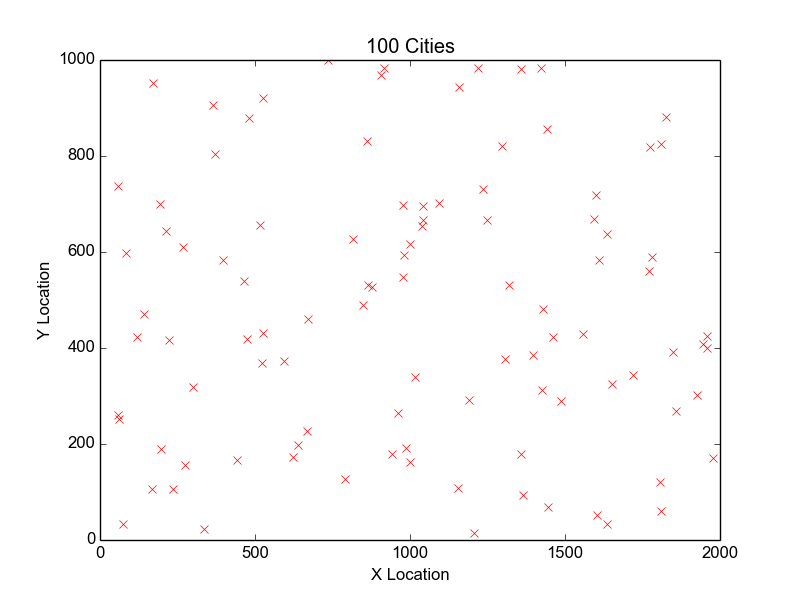
\includegraphics[width=0.9\textwidth]{100cities.png}
	    \caption{100 cities plot}
	    \label{fig:100cities}
    \end{minipage}\hfill
	\begin{minipage}{0.5\textwidth}
	    \centering
	    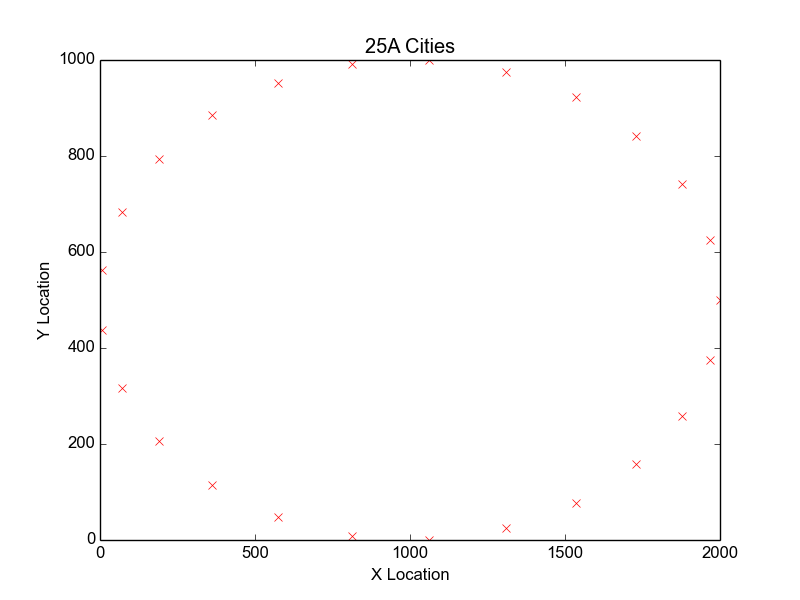
\includegraphics[width=0.9\textwidth]{25cities_A.png}
	    \caption{25 cities plot}
	    \label{fig:25Acities}
    \end{minipage}\hfill
\end{figure}

%!TEX root = HW2.tex





\section{Algorithm Explanation}
\subsection{Simulated Annealing}
% In this work, a basic version of Simulated Annealing is implementated.  
\begin{itemize}
\item s = InitialGuess()
\item For i < TOTALITERATIONS:
	\begin{itemize}
	\item sNew = NeighborSol(s)
	\item s = TempSelect(s, sNew, Temp)
	\item DecreaseTemp(Temp)
	\end{itemize}
\item FinalSolution = s
\end{itemize}

\textbf{InitialGuess} -- Intial solution generated randomly \\
\textbf{TOTALITERATIONS} -- Number of solutions to try \\
\textbf{NeighborSol} -- Generate a succesor state to $s$ by switching the order of two adjacent cities in $s$ \\
\textbf{TempSelect} -- Selects a solution between the two presented based on the temperature.  The best solution is probabilistically choosen based on the temperature.  The higher the temperature the more likely the next solution is choosen at random. \\
\textbf{DecreaseTemp} -- Decrases the temperature such that it ends at 0 (always choosing the better solution) when the maximum number of iterations is reached. 

\subsection{Evolutionary Algorithm}
% In this work, a 
\begin{itemize}
	\item POP = InitialGuess(POP\_TOT)
	\item For i < TOTALITERATIONS:
		\begin{itemize}
			\item POP\_SEL = ChooseParents(POP)
			\item CHILD = PerturbPopulation(POP\_SEL)
			\item POP = SelectPop(CHILD, POP)
		\end{itemize}
	Soltuion = Min\_Value(Pop)
\end{itemize}

\textbf{InitialGuess} -- Initial population of solutions generated randomly \\
\textbf{TOTALITERATIONS} -- Number of generations \\
\textbf{ChooseParents} -- Epsilon-greedy choose best solutions in population based on some amount of noise \\
\textbf{PerturbPopulation} -- Finds neighbor solutions based on choosen parents.  The amount of variation to original solution is based on an amount of noise.  Variation is implemented as the number of switches between neighboring cities in a solution.  Higher noise means more neighboring cities will be switched. \\
\textbf{SelectPop} -- Choose the best solutions from the original population and mutated children.  The resulting number of solutions is equal to the starting population size. \\
\textbf{Min\_Value} -- From a given population, returns the member that has the best solution value. \\

In this assignment, Population size was 10.  Number of children produced each round was 5.  Noise was decreased from 1 to 0 based on current iteration number.  For this algorithm, the total number of iterations was choosen as 1,000.  This is ten times less than the other two approaches in order to have a similar number of total generated solutions.  

\subsection{Monte Carlo Tree Search}
The implementation used in this assignment is not optimized.  As a result, it has slow run times but is able to find solutions. \\
\textbf{Main Algorithm}
\begin{itemize}
	\item InitializeTree()
	\item For i < TOTALITERATIONS:
		\begin{itemize}
			\item Parent = PickParent(Tree)
			\item Node = PickChild(Parent)
			\item Leaf\_Value = DescendTree(Node)
			\item BackPropogateValue(Leaf\_Value)
		\end{itemize}
\end{itemize}

\textbf{DescendTree}
\begin{itemize}
	\item If Node has Children
	\begin{itemize}
		\item Node = PickChild(Node)
		\item DescendTree(Node)
	\end{itemize}
	\item Else: PlayOut()
\end{itemize}

\textbf{InitializeTree} -- Initializes tree structure.  Nodes are initialized with best value to promote exploration. \\
\textbf{TOTALITERATIONS} -- Number of solutions to try \\
\textbf{PickParent} -- Probabilistically chooses the first node of the tree based on value. \\
\textbf{PickChild} -- Probabilitically choose a child from a node.  If the node does not exist, create it. \\
\textbf{DescendTree} -- Subfunction that continues to descend the tree in a probablisitic manner based on node value \\
\textbf{PlayOut} -- Determines value of a node on its first visit.  The remaining cities are choosen at random to create a valid path.  Returns the value of the full path. \\
\textbf{BackPropogateValue} -- Value of the current node is pushed to the parent.  The parent adds the new value to its current value based on the total number of visits.  For example, if a parent has been visited once before, then $(Old\_Value * Number\_Of\_Visits + New\_Child\_Value) / (Number\_Of\_Visits + 1)$.  This is effectively an average value of the node based on all explored solutions.  A node with a good value is more likely to lead to a good solution than a node with a worse value.


%!TEX root = HW2.tex
\section{15 Cities}
\subsection{Results}
For 15 cities, the algorithms all perform decently well.  The evolutionary algorithm was able to find the best solution.  SA and MCTS are both able to find near optimal algorithms.  EA takes significantly longer than the other two algorithms.  Additionally, SA has the largest variance of each iteration of all the methods between runs while EA and MCTS have similar amounts of variance in each iteration during the search process.    

One reason for EA's better performance is that it holds many more solutions in memory at a time and can compare them against each other.  The other methods hold only one or two solutions at a time and make comparisons based on those two only.  In this implementation of EA, the best solution can never be removed.  If an optimal solution is discovered, it will not be discarded which is true for MCTS, but not SA.  In all cases, EA decreases in distance the quickest.  This may be due to having acces to many solutions that it can quickly hone in on a promising solution.  Although, this may be problematic later on if this is a local minimum.

SA may struggle to get to the optimal solution if it is currently at a state that is near the optimal solution.  If more than a single switch of two consecutive states is requried to achieve a solution, then SA is unlikely to get to that solution.

MCTS has to hold a tree structure which can get quite large in memory.  Each iteration can add a new node to the tree and requires several calculations to update the tree with every iteration.  

% Put table with run time and solution quality results
\begin{table}[H]
\centering
\label{my-label}
\begin{tabular}{|c|c|c|c|c|c|}
\hline
Algorithm               & \begin{tabular}[c]{@{}c@{}}Total Solutions\\ Generated\end{tabular} & \begin{tabular}[c]{@{}c@{}}Average Min\\ Distance\end{tabular} & St Dev & \begin{tabular}[c]{@{}c@{}}Average\\ Run Time (s)\end{tabular} & St Dev \\ \hline
Simulated Annealing     & 10,000                                                              & 7,685                                                          & 994     & 4.72e-6                                                    & 3.8e-6 \\ \hline
Evolutionary Algorithm  & 10,000                                                              & 5,861                                                          & 359    & 4.39                                                       & 0.17   \\ \hline
Monte Carlo Tree Search & 10,000                                                              & 5,916                                                          & 289    & 2.19                                                       & 0.08   \\ \hline
\end{tabular}
\caption{Comparison of Solution Quality and Run Time for Each Method with 15 Cities}
\label{tab:15Comparison}
\end{table}


% insert image of example solutions found by search

\begin{figure}[H]
	\centering
    \begin{minipage}{0.45\textwidth}
        \centering
        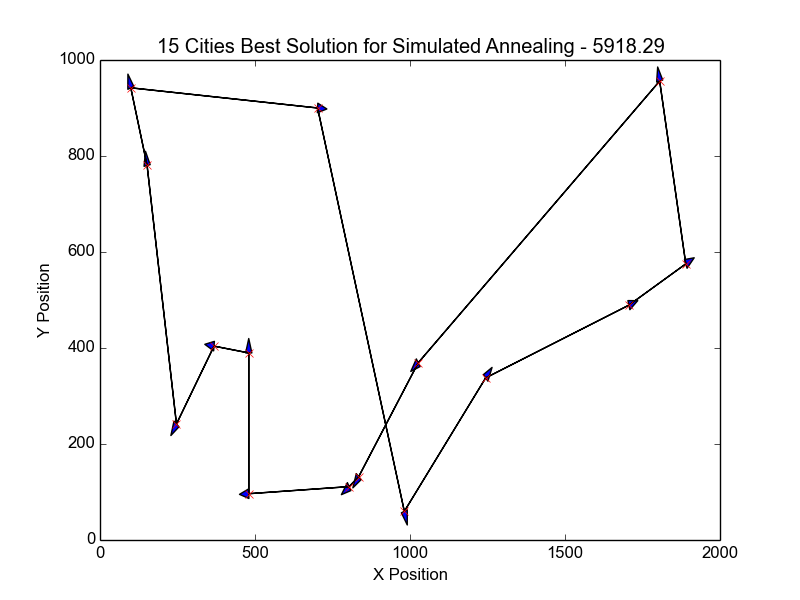
\includegraphics[width=0.9\textwidth]{15City_SA.png} % second figure itself
        \caption{Best Solution for 15 Cities with Simulated Annealing}
        \label{fig:15city_SA}
    \end{minipage}\hfill
    \begin{minipage}{0.45\textwidth}
        \centering
        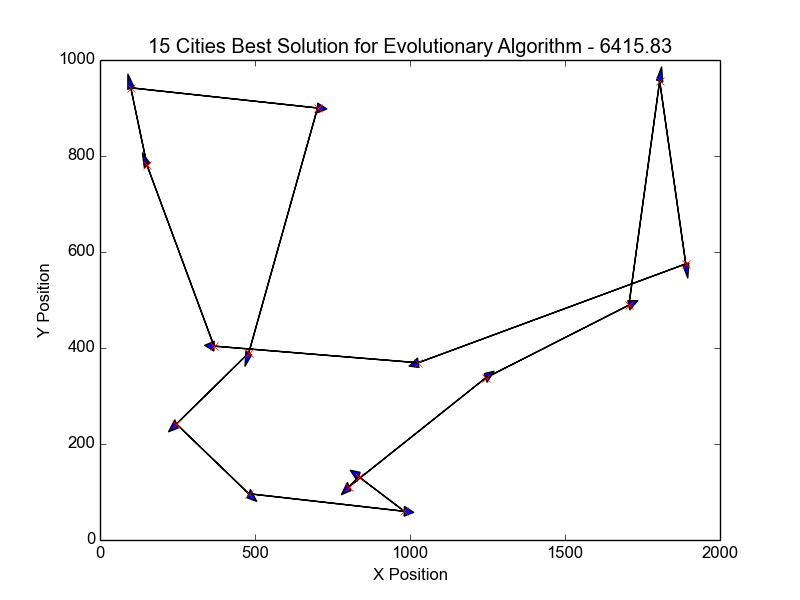
\includegraphics[width=0.9\textwidth]{15City_EA.png} % first figure itself
        \caption{Best Solution for 15 Cities with Evolutionary Algorithm}
        \label{fig:15city_EA}
    \end{minipage}\hfill
    \begin{minipage}{0.45\textwidth}
        \centering
        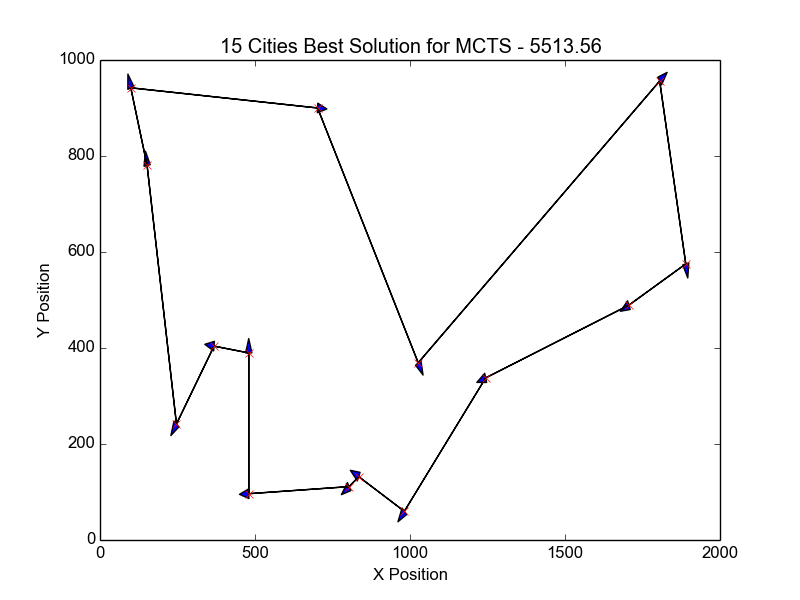
\includegraphics[width=0.9\textwidth]{15City_MCTS.png} % third figure itself
        \caption{Best Solution for 15 Cities with MCTS}
        \label{fig:15city_MCTS}
    \end{minipage}\hfill
    \begin{minipage}{0.45\textwidth}
		\centering
		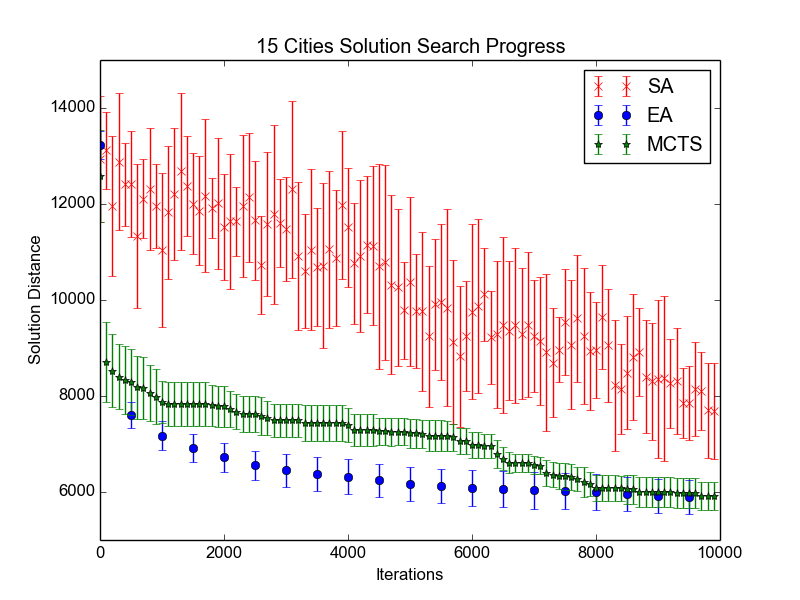
\includegraphics[width=0.9\textwidth]{15City_Solutions.png}
		\caption{Solution Progression for 15 Cities}
		\label{fig:15city_Solution}
    \end{minipage}\hfill
\end{figure}

% \section{Question 1}
\subsection{Part A}
The number of hidden units primarily affects the speed that the model converges at.  Looking at the figure below, 20 hidden units appears to be the best number.  However, by the third epoch, 5 hidden units has similar performance and by the ninth epoch, 100 hidden units has converged.  This is likely because the function to classify the outputs is relatively simple.  For a more complex problem, the number of hidden units would also affect the accuracy of the classifier.  However, having too many hidden units can allow the model to overfit.  This can be more clearly seen in Part B.
\begin{figure}[H]
	\centering
	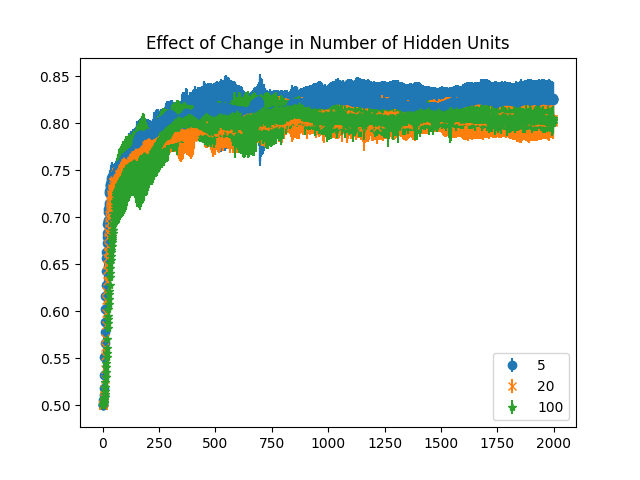
\includegraphics[width=0.6\textwidth]{../train1/hidden_units.png}
	\caption{Effect of changing number of hidden units}
\end{figure}

\subsection{Part B}
The biggest effect that training time has is that as training time increases, performance begins to degrade.  The model is overfitting to the training set which is making it less generalizable.  As a result, performance degrades on the test set.  In an extreme case, too little training time will cause the model not to achieve maximum performance, but for this data set, that is less than 5 epochs.  The results of short training time can be seen in Part A.
\begin{figure}[H]
	\centering
	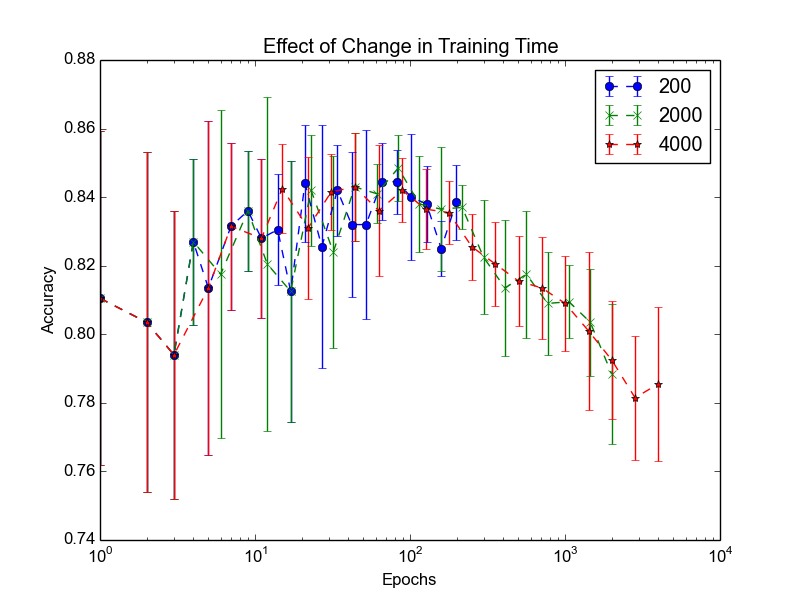
\includegraphics[width=0.6\textwidth]{../train1/epochs.png}
	\caption{Effect of changing traning time}
\end{figure}

\subsection{Part C}
The size of the learning rate affects how quickly the classifier converges.  With very small steps, the classifier takes a long time to converge.  With very large steps, the classifier diverges and always performs poorly.  An appropriate step size allows for convergence to happen in a reasonable amount of time.
\begin{figure}[h]
	\centering
	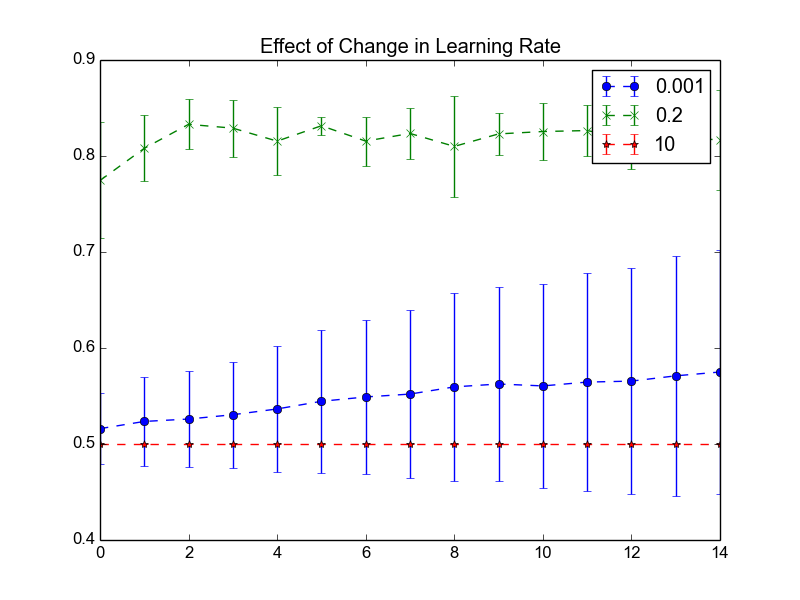
\includegraphics[width=0.6\textwidth]{../train1/learning_rate.png}
	\caption{Effect of changing learning rate}
\end{figure}

\subsection{Part D}
I found an interesting bug (feature?) in Python when using multiprocessing.  The cause (I think) is that because the processes spawn so quickly, they all use the same machine time to generate their random weight initializations.  This results in all of the newtorks having the same results.  This is even more surprising since the data is shuffled for every epoch.  I believe that again the shuffling was happening the same for all of the trials.  I was eventually able to cause the weights to be different by seeding the generator with different values for each trial.  An intersting problem that only occurs when using multiprocessing.

Some other parameters that the can change convergence time and network performance are the initialization weights of the network and shuffling the data during processing.
\begin{figure}[h]
	\centering
	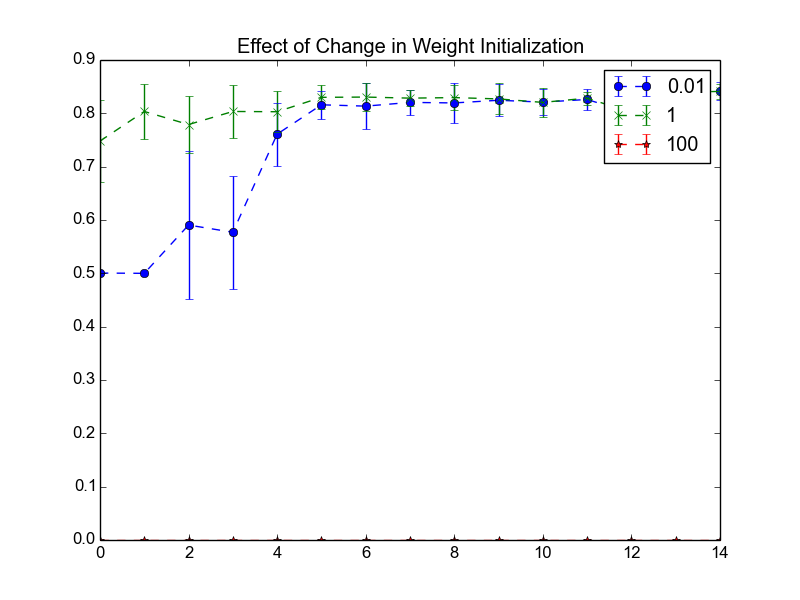
\includegraphics[width=0.6\textwidth]{../train1/weights.png}
	\caption{Effect of classifier on different test data sets}
\end{figure}


\subsection{Part E}
Different data sets have similar performance.  Performance on dataset two appears to be the best.  Test set 2 has the closest distribution of passes and fails as the model.  Although, this does not completely explain the difference.  The biggest issue is likely that the training data sets differs the least from set 2.  Set 1 has many more passes than fails.  This might suggest that the model tends to predict more passes than fails (false positives).  Since Set 3 has more fails than passes, this bias may also explain the poorer performance of the classifier on the third data set.
\begin{figure}[h]
	\centering
	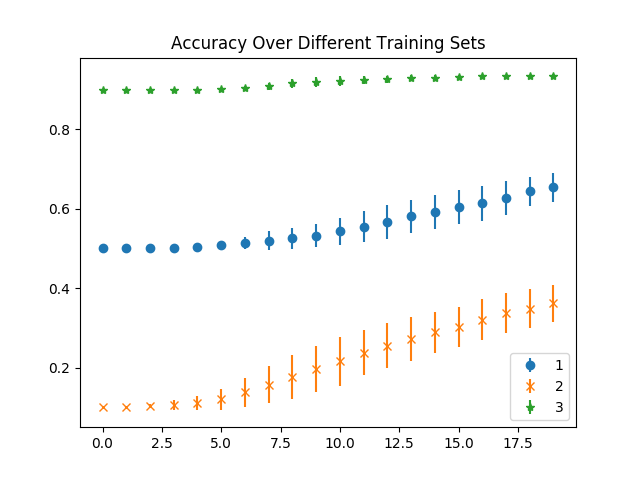
\includegraphics[width=0.6\textwidth]{../train1/data_sets.png}
	\caption{Effect of classifier on different test data sets}
\end{figure}

% \section{Question 2}
\subsection{Part A}
\begin{figure}[H]
	\centering
	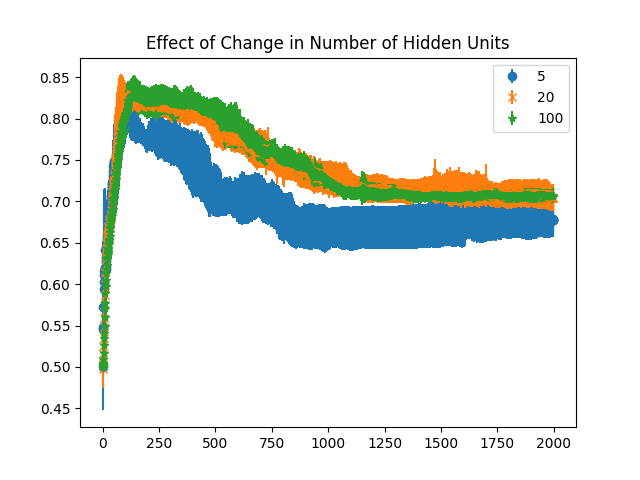
\includegraphics[width=0.6\textwidth]{../train2/hidden_units.png}
	\caption{Effect of changing number of hidden units}
\end{figure}

\subsection{Part B}
\begin{figure}[H]
	\centering
	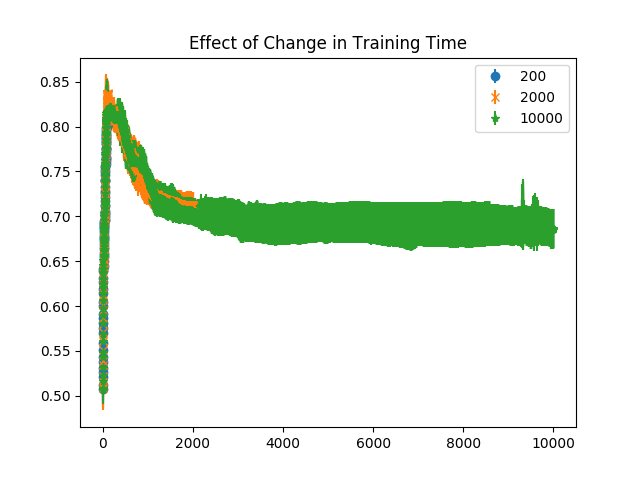
\includegraphics[width=0.6\textwidth]{../train2/epochs.png}
	\caption{Effect of changing traning time}
\end{figure}

\subsection{Part C}
\begin{figure}[H]
	\centering
	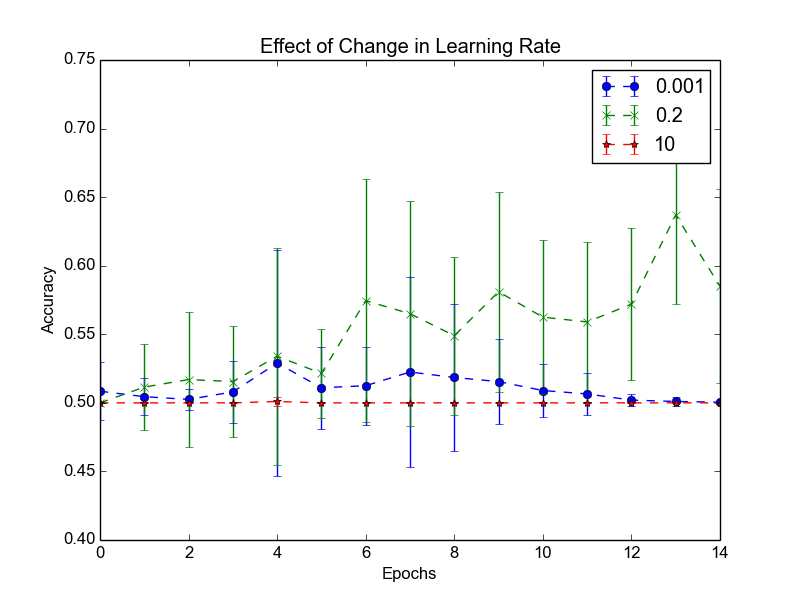
\includegraphics[width=0.6\textwidth]{../train2/learning_rate.png}
	\caption{Effect of changing learning rate}
\end{figure}

\subsection{Part E}
\begin{figure}[H]
	\centering
	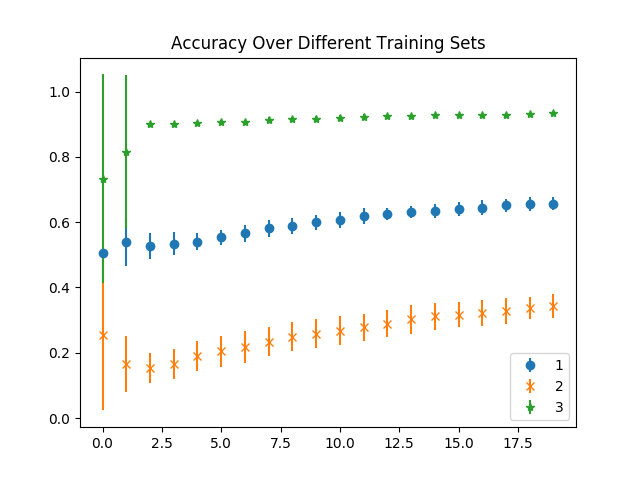
\includegraphics[width=0.6\textwidth]{../train2/data_sets.png}
	\caption{Effect of classifier on different test data sets}
\end{figure}

\bibliographystyle{unsrt}
\bibliography{HW2}

\end{document}	